\section{Language Buzzwords}
\label{sec:buzzwords}

Through our prototype of LANCOM we intend to demonstrate a common high -
  level language for router and firewalling configuration.Particularly,
  we attempt to design a language which maintains separation of network
  topology and routing information description from firewalling and security
  policies.Using role based access control \cite{bartal99firmato}
 , we intend to configure any policy on any routing and networking topology
  description with minimal modifications. We borrow the concept of encapsulation
   from object oriented programming to describing the network entities and roles as objects.
  These objects are collection of attributes and methods. Attributes of the objects of classes
   describing policies and roles maybe used to act upon attributes of objects of 
  classes describing networking topology.

\begin{itemize} 
 
 \item \noindent {\bf Ease of use}: Commercial routers and firewalls have 
    their own syntax constructs and peculiarities. A system administrator 
    needs to expend time and effort in in learning such syntices.A small sized 
    networks may deploy devices from various vendors. Configuring all such devices,
    keeping in mind the syntactic and semantic peculiarities of the
    configuration languages of all these devices, adds up to the ever increasing 
    and daunting responsibilities of the human
    administrator. 

 \begin{figure}[ht] 
 \label{fig:ease_of_use}
  %\centering 
 \begin{center}
  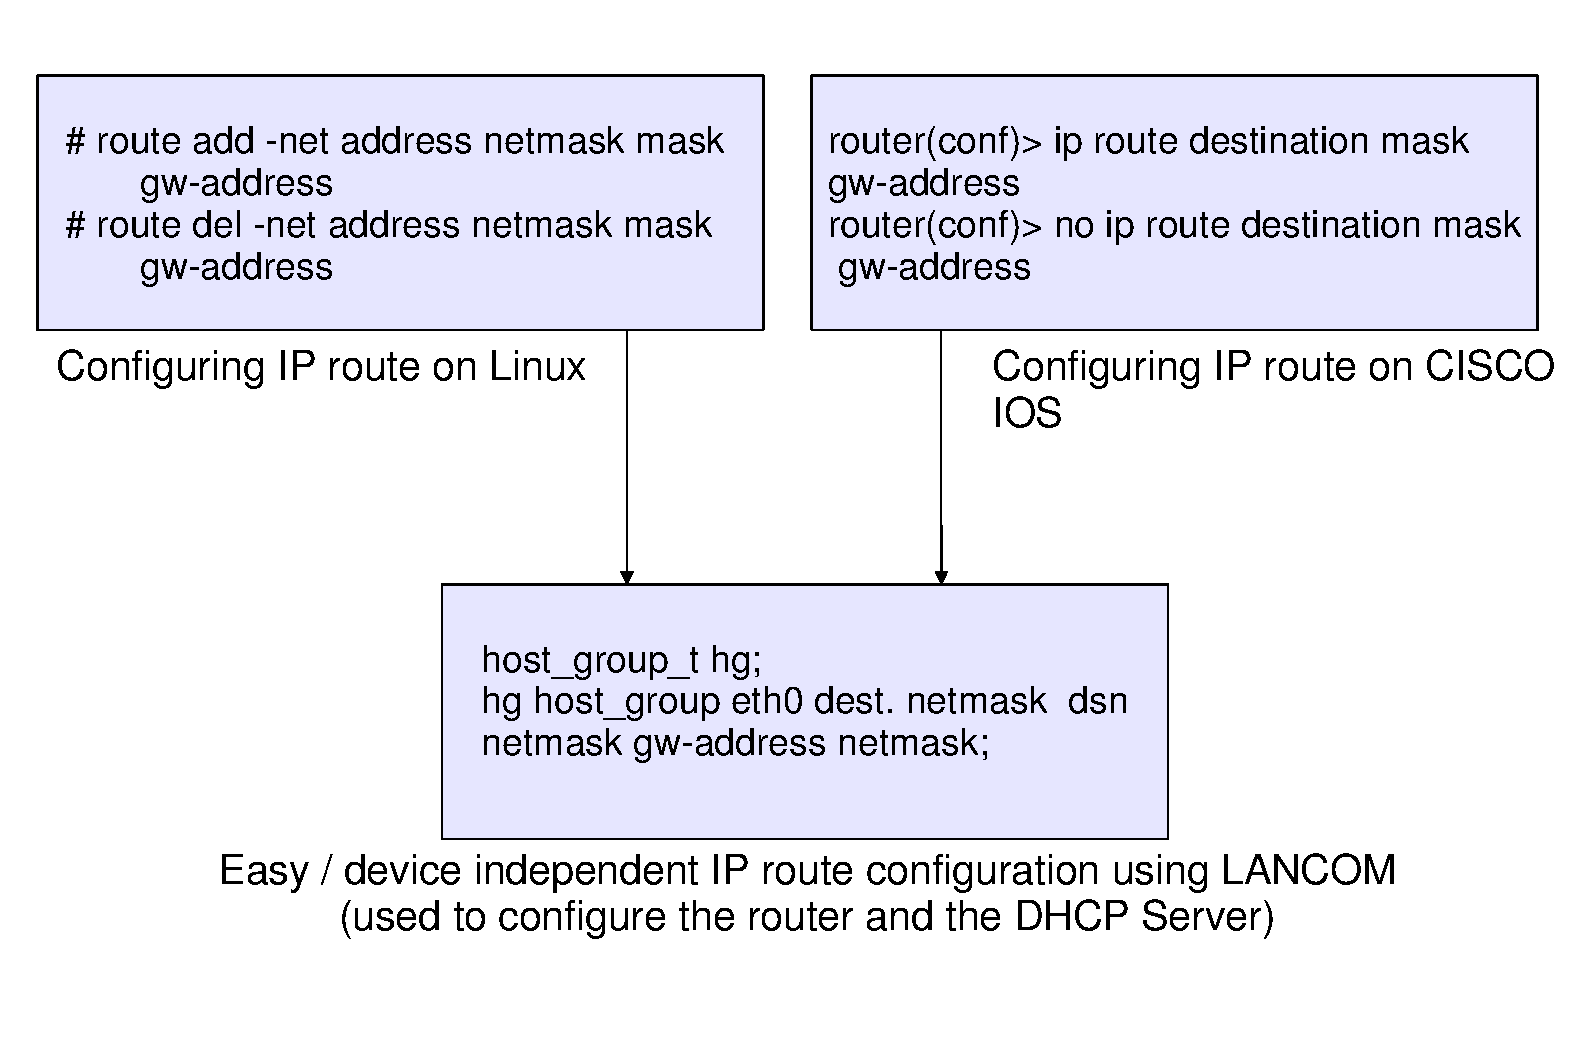
\includegraphics[scale=0.35]{figs/ease_of_conf.pdf}
  \end{center}
  \smallcaption{LANCOM makes it easy for a system administrator to write device
      independent routing and firewalling configurations}
   \end{figure}

   

%Let us take the example of a small network of linux PCs connected with a
%Cisco router and ethernet hubs. n order to statically configure a routing table,
%the user needs to f %
%amiliarize himself with the routing commands on linux OS as well as the
%routing command on Cisco 's IOS. And these sets of commands are different. Imagine the complexity of co% nfiguring a network with several hundreds of PCs running different operating systems and supporting different routers! 

Through LANCOM, we aim at relieving administrators the responsibility of learning the configuration syntices of the various routing and firewalling devices his organization uses. It aims to be a common language, that can be used to configure any interface or firewall in the network. Figure ~\ref{fig:ease_of_use} shows how LANCOM can be replaced by multi-lingual configutation syntices. This saves the user the time and effort needed to learn multiple commands on different systems and allows them to focus on configuring topologies and designing security policies.

\item \noindent {\bf Portability}: We aim at providing a common high-level interface across multiple systems. It enables unified management of networking elements from different vendors/manufacturers. It may ideally ease the transition of an organization' s switching networking products from one vendor to another. 

\item \noindent {\bf Flexibility}: We propose separation between security policy description from the
	network topology description. We aim to provide the users with flexibility of configuring firewalls,
	``independent '' of specifying the networking topology and routing
	information. Moreover, the very nature of the grammar being relatively ``small'',
	promises modularity and granularity. 

\item \noindent {\bf Scalability}: LANCOM would scale across various network sizes.
      Since we propose a relatively ``small'' but robust grammar,
      LANCOM maybe used for describing the network topology, routing information and security policy,
      {\bf regardless of the number of devices attached}. The language shall not impose restrictions on 
      the magnitude of the network. 

\begin{figure}[ht] 
\label{fig:scalability}
    %\centering 
\begin{center}

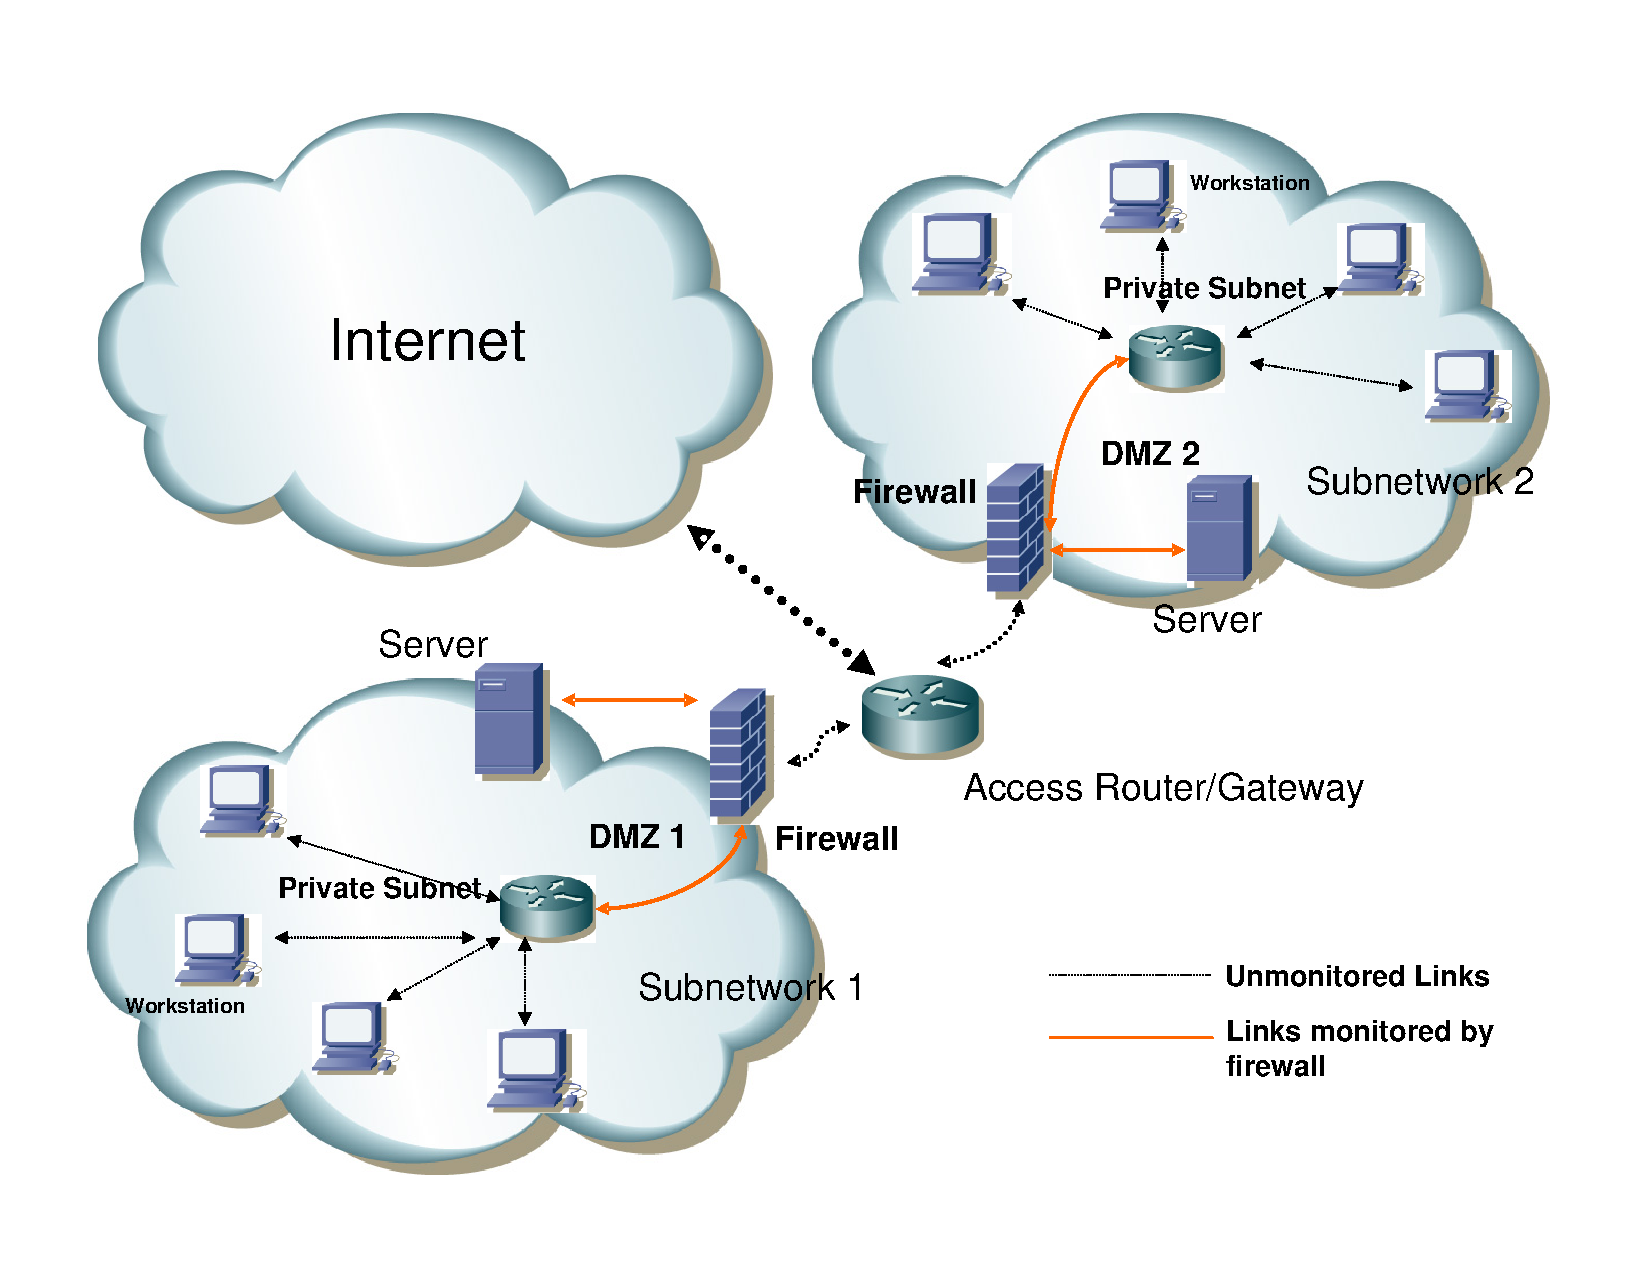
\includegraphics[scale=0.3]{figs/scalability.pdf}
\end{center}
\smallcaption {LANCOM may make configuration independent on the size of the network and
	the underlying toplogy}
\end  {figure}
     %Our language is mainly intended to be used by the System Administrators or in the field of System and Security 
%   Management for configuring routers and firewalls in a large company setup.In such a scenario Scalability will play a very important 
%  role as there can be a large set of inter connected systems on a network overlay.Our language can be used to configure � �n � �number 
%  of computers and routers simultaneously and hence reducing the overhead involved.The language will not impose any restrictions on the 
%  size of the network and will be scalable to accommodate networks as they grow larger or smaller. 


\item \noindent {\bf Reliability}: The LANCOM compiler shall produce configuration files that can be used
	  directly to configure systems.We hope to produce, to the best of our knowledge and abilities,
	  parsers and semantic analyzers which would generate configurations
	  free from security bugs and misconfiguration. 




\item \noindent{\bf Re-usability}: The final, and maybe the most important reason for us
	to design LANCOM, is to reduce the workload and overhead involvedn
          in configuring various firewalls and routers.We plan to add re-usabilty 
          to the language through constructs such as macros and
	  procedure calls.

 \end{itemize}

That said, we show give an overview of grammar used by LANCOM and how it can be used 
by administrators to generate configuration, without knowledge of the vendor specific language syntax.
